\hypertarget{ux446ux435ux43bux44c-ux440ux430ux431ux43eux442ux44b}{%
\section{Цель
работы}\label{ux446ux435ux43bux44c-ux440ux430ux431ux43eux442ux44b}}

Получить опыт работы с Git. Создать аккаунт; подключить репозиторий к
Github; Пройти первичную конфигурацию; провести конфигурацию git-flow.

\hypertarget{ux437ux430ux434ux430ux43dux438ux435}{%
\section{Задание}\label{ux437ux430ux434ux430ux43dux438ux435}}

\begin{itemize}
\item
  Сделать отчет по предыдущей работе в формате Markdown.
\item
  Предоставить в 3-х форматах: pdf, md and docx.
\end{itemize}

\hypertarget{ux432ux44bux43fux43eux43bux43dux435ux43dux438ux435-ux43bux430ux431ux43eux440ux430ux442ux43eux440ux43dux43eux439-ux440ux430ux431ux43eux442ux44b}{%
\section{Выполнение лабораторной
работы}\label{ux432ux44bux43fux43eux43bux43dux435ux43dux438ux435-ux43bux430ux431ux43eux440ux430ux442ux43eux440ux43dux43eux439-ux440ux430ux431ux43eux442ux44b}}

\hypertarget{ux441ux43eux437ux434ux430ux435ux43c-ux430ux43aux43aux430ux443ux43dux442-github}{%
\subsubsection{1. Создаем аккаунт
github}\label{ux441ux43eux437ux434ux430ux435ux43c-ux430ux43aux43aux430ux443ux43dux442-github}}

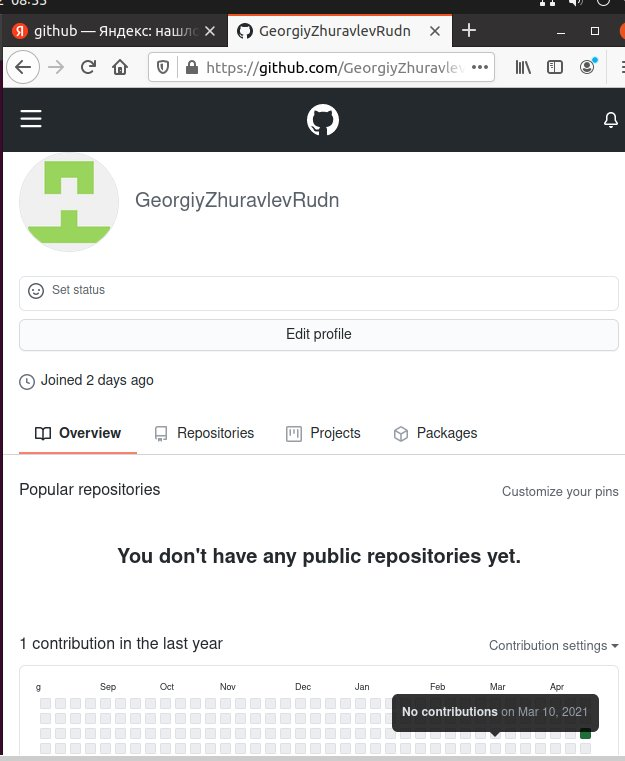
\includegraphics{scrsht/1.jpg} \#\#\# 2. Генерируем ключ для настройки
VCS. 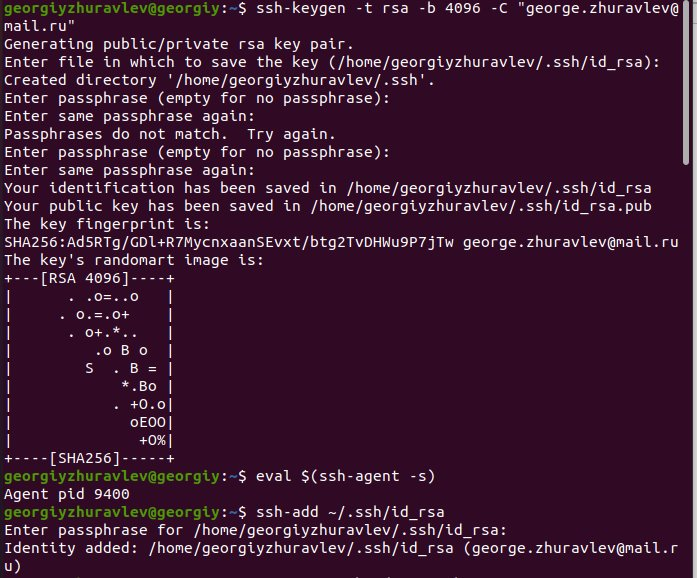
\includegraphics{scrsht/2.jpg} \#\#\# 3. Добавляем сгенерированный
ключ. 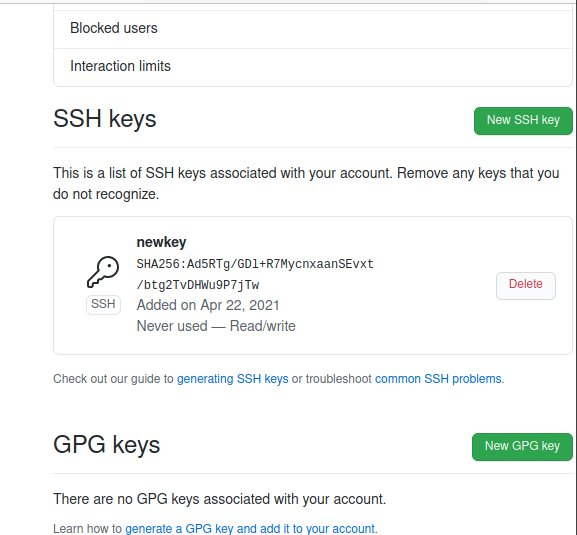
\includegraphics{scrsht/3.jpg} \#\#\# 4. Приступаем к созданию
репозитория и файлов. 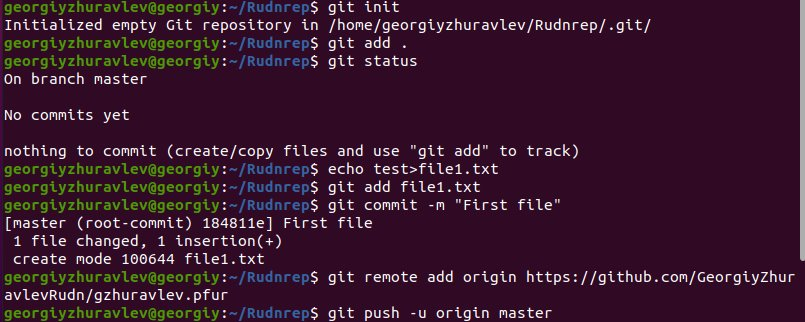
\includegraphics{scrsht/4.jpg} \#\#\# 5. Добавляем
лицензию 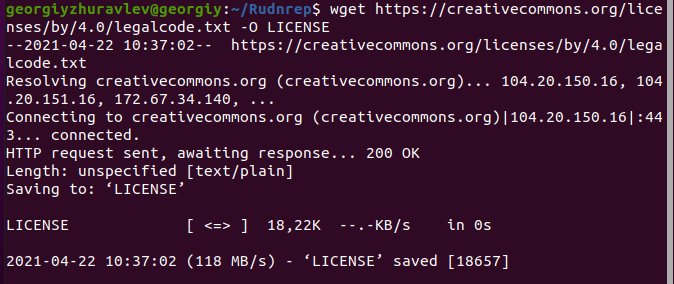
\includegraphics{scrsht/5.jpg} \#\#\# 6. Добавляем игнорируемый
файл ( с помощью vs code). 
\includegraphics{scrsht/6.jpg} \#\#\# 7.
Инициализируем git flow. 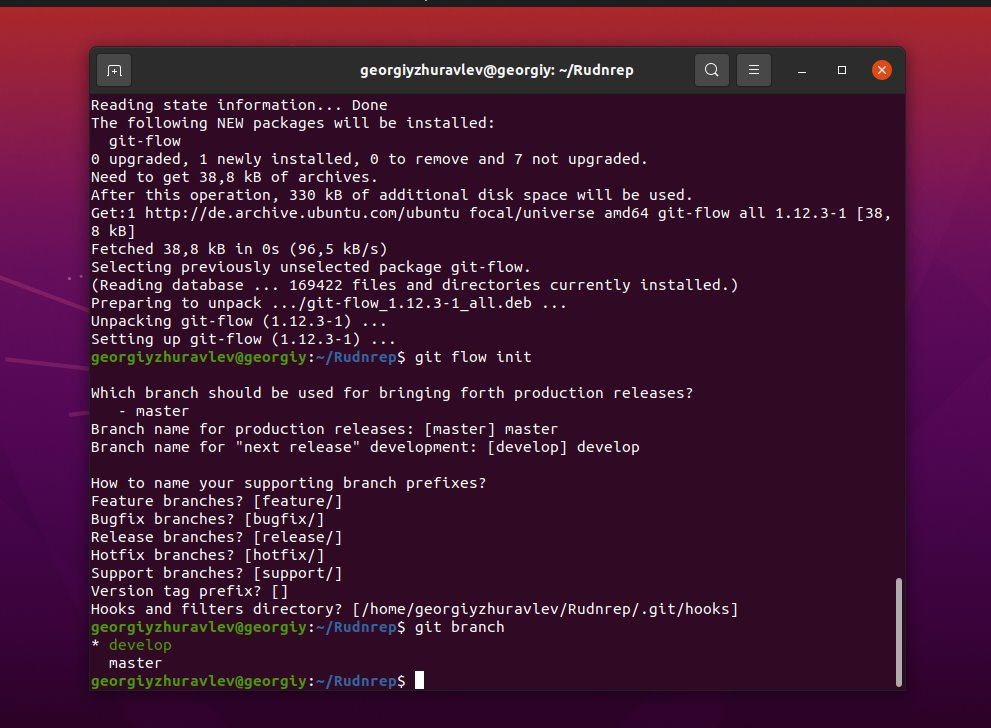
\includegraphics{scrsht/7.jpg} \#\#\# 8.
Добавляем релиз и загружаем на Github. 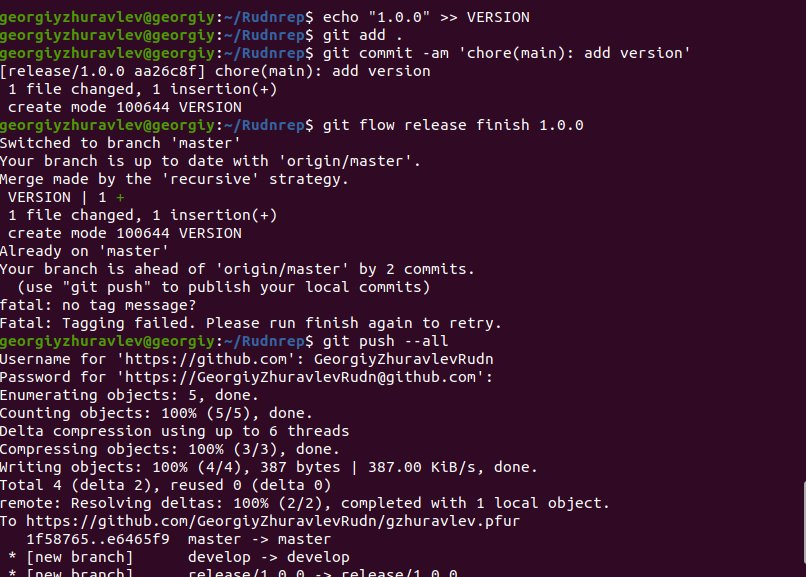
\includegraphics{scrsht/8.jpg}

\includegraphics{scrsht/9.jpg} 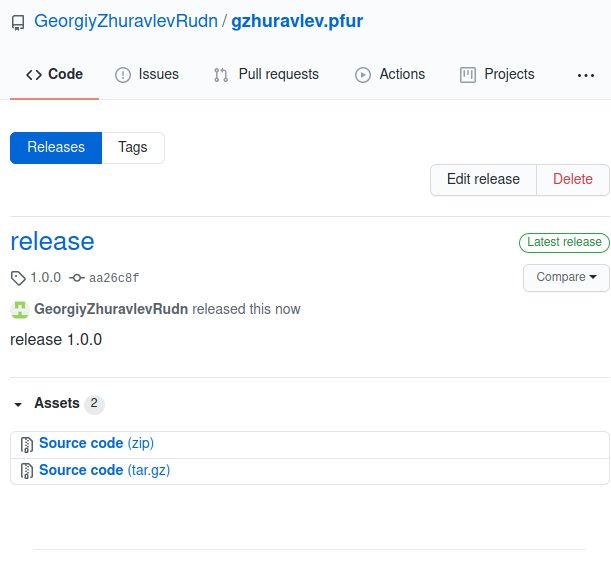
\includegraphics{scrsht/10.jpg} \#\#\# 9.
Получившиеся результаты(ветви + данные). 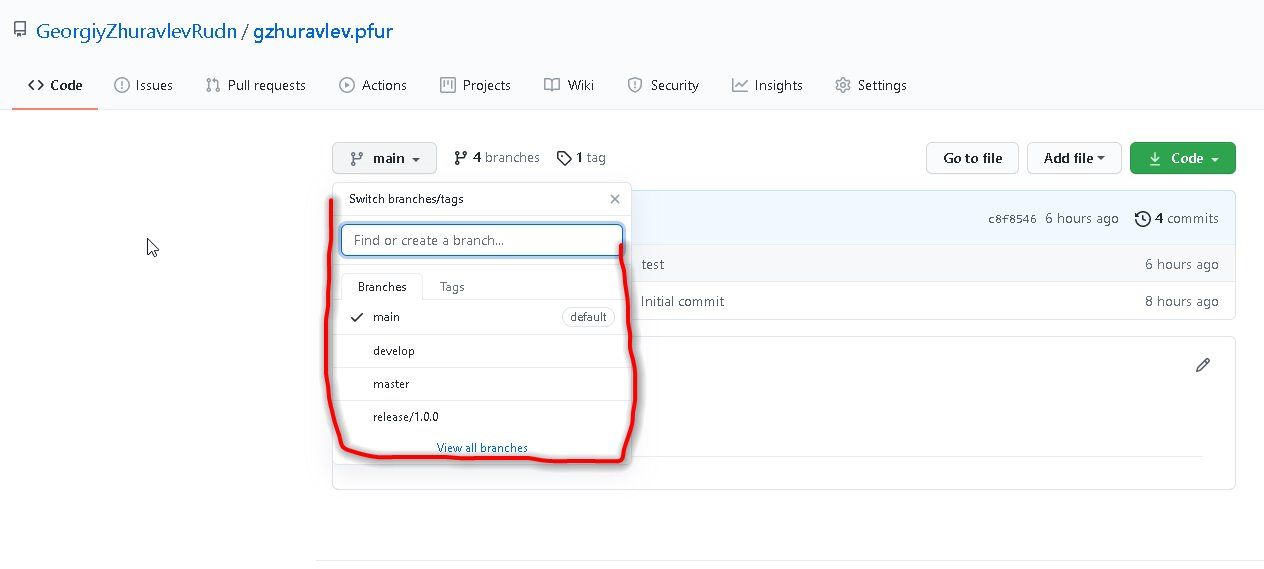
\includegraphics{scrsht/11.jpg}

\hypertarget{ux432ux44bux432ux43eux434}{%
\section{Вывод}\label{ux432ux44bux432ux43eux434}}

Благодаря этой лабораторной работе, я научился: создавать репозитории,
создавать файлы и проходить процесс подтверждения, загружать файлы в
репозиторий git, делать релизы и создавать ветви.

\hypertarget{ux43aux43eux43dux442ux440ux43eux43bux44cux43dux44bux435-ux432ux43eux43fux440ux43eux441ux44b}{%
\section{Контрольные
вопросы}\label{ux43aux43eux43dux442ux440ux43eux43bux44cux43dux44bux435-ux432ux43eux43fux440ux43eux441ux44b}}

\begin{enumerate}
\def\labelenumi{\arabic{enumi}.}
\item
  VCS -- ПО для облегчения работы с изменяющиеся информацией(хранит
  изменяющиеся версии; может быть изменена разными людьми, если проходит
  работа над совместным проектом). VCS предназначена для удобства
  использования в проектах, например один человек написал некоторый код,
  который хочет поместить в основную ветвь проекта, его коллеги могут
  проверить и сделать заметки в виде комментариев.
\item
  Хранилище -- основное место хранения; Commit -- подтверждение всех
  изменений и тп., для дальнейшей загрузки в репозиторий; History --
  история изменения; Рабочая копия -- действительные папка с файлами.
\item
  Централизованные системы контроля представляют собой приложения типа
  клиент-сервер;( 1 основной репозиторий)(SVN) Распределенные системы
  контроля версий позволяют хранить репозиторий (его копию) у каждого
  разработчика, работающего с данной системой.( множество репозиториев,
  взаимодействующих с сервером)(Git)
\item
  Создание репозитория \textasciitilde\textgreater{} создание/добавление
  файлов в локальную файловую систему \textasciitilde\textgreater{}
  добавление в локальный репозиторий \textasciitilde\textgreater{}
  подтверждение добавления \textasciitilde\textgreater{} загрузка в
  онлайн репозиторий.
\item
  \begin{itemize}
  \tightlist
  \item
  \end{itemize}
\item
  \begin{itemize}
  \tightlist
  \item
  \end{itemize}
\item
  Git add -- adds a file to the staging area; git commit- opens chosen
  git editor or git commit -m ``message''(commitment with a message);
  git push -- pushes files to repository; git pull -- downloads/ changes
  files from repository; git branch -- shows branches; git status --
  status of your process; git rm ``\,''- removes a file/es; and so on.
\item
  Создание файла в репозитории( лок.); загрузка файлов на удалённый
  репозиторий(удал.)
\item
  Ветви -- специальные разделения дерева, которые нужны для удобства
  использования git, например для дальнейшего merg'a.
\item
  ``git editor''.gitignore \textasciitilde\textgreater git add
  .gitignore\textasciitilde\textgreater git commit; Игнорирование нужно
  для исключения ненужных файлов/ файловых систем/ тп. из области
  работы.
\end{enumerate}
